\documentclass[a4paper]{article}

\usepackage[english]{babel}
\usepackage[utf8x]{inputenc}
\usepackage[colorinlistoftodos]{todonotes}
\usepackage{fullpage}
\usepackage{color}
\newcommand{\comment}[1]{\textcolor{red}{#1}}
\title{Evolution III: Kalendr}
\author{Ellango Jothimurugesan, David Liu, Pritam Mathivanan, and Benson Tran}

\begin{document}
\maketitle

\begin{abstract}
This is not a research paper, but having an abstract section makes the report look polished. In any case, in this report, we are going to discuss our design choices for our calendar web application \textit{Kalendr}\comment{---}spoofing Silicon Valley startups\comment{---}using Django and Angular.
\end{abstract}

\section{Introduction}

In this report we will provide a retrospective on our previous design choices and their impact on completing features for this evolution, further providing insight on where such design choices made implementation feasible or a complete hassle. Moreover, we will discuss our design choices for this current evolution and elaborate on their strengths and weaknesses. In terms of front end development, we will continue to elaborate on how the Angular framework has consistently provided multiple avenues for design choices, making front end implementation relatively seamless yet convoluted in some cases. In terms of back end development, we will continue to discuss the limitations of the Django REST famework and discuss how implementations in previous evolutions have complicated development for the current evolution. Lastly, we expand on our choices\comment{---}whether they be in the scope of frameworks, languages, database design, UI design, documentation, or teamwork\comment{---}to help us be more cognizant of better ways of tackling future evolutions.

\section{Retrospective}

By the third evolution there was a clear disparity in the difficulty of implementation between the front end and the back end. The second evolution proved to be more front end heavy in terms of developing a Social Bar, a PUD view, and implementing different forms and views within one web page. Each front end feature is essentially a module, each with a controller, service, and directive. Although there may have been some hacky solutions within the front end, Angular's inherent modularity helps tremendously with the bookkeeping - hacky solutions are slightly more sustainable as such modularity reduces the number of dependencies among modules. However, back end development proved to be more challenging this time around.

In terms of backend development, we were continually discovering limitations with the Django REST framework. Despite these limitations we were still able to develop robust and flexible viewsets. Unfortunately, to add to the woes, hacky solutions from the first couple of evolutions were now catching up with us. Date and time manipulations and discrepancies between the front end and the back end slowed development and added frustration.

\subsection{Front End Design Choices and Issues - Angular.js}

Angular.js continues to make dynamic DOM implementation relatively simple with features such as \textit{ng-init, ng-model, ng-repeat,} and \textit{ng-show}. We continue to use these features throughout Evolution III; however, in some ways, one can make that argument that we have become too 'reliant' on particular ng-elements. 


\subsubsection{Breaching Encapsulation}

As alluded to in the previous evolution, Angular's ability for two-way binding between the DOM and controller allows the programmer to more easily undermine the concept of encapsulation between the DOM and the controller. Working on large projects with growing bookkeeping pains, it may be difficult for all members to be on board with which variables and functions should stay private within the scope of the controller and not exposed to the client.

Although this idea of encapsulation between the DOM and controller can be superficially rectified via thorough commenting and religious refactoring of controllers, encapsulation is still breached by controller-to-controller and DOM-to-DOM data-passing.

Angular provides the programmer with objects \textit{scope and rootScope} each with functions \textit{.broadcast(), .watch(), and .emit()}. The purpose of these objects and functions is to propagate triggering events from one controller to another. Pressing a button on a form that triggers an update on another page is a canonical use case. It's noted as good practice to \textit{not} pass data in these triggering events, but instead to perform a service GET or POST call.

Within Angular, services are used to make calls to the server to update modules within any controller. These services can be injected and called from any controller. A naive programmer who passes data via \textit{.broadcast() and .emit()} calls and service \textit{http} calls simply convolutes the controller by providing superfluous references to the same fields.

Lastly, DOM-to-DOM data-passing is introduced in our project via the use of the \textit{ng-dialog-data} attribute of the \textit{ng-dialog} directive. The purpose from the \textit{ng-dialog} is maintain a dynamic, one-page web application by passing information into popups. Information from popups is generally passed back to the main controller via broadcasting or saving to the database via a \textit{http} service call. Continuing with the trend, DOM-to-DOM data-passing convolutes bookkeeping. In some cases, rather than using \textit{ng-dialog-data}, we simple perform a GET request when a popup is instantiated.

Although we lauded Angular's many powerful objects and tools in the previous evolution's writeup, we've become cognizant of the many bookkeeping issues that follow with our naive use cases of data-binding and data-passing. 


\subsection{Back End Design Choices - Django and Django REST Framework}
As a powerful and widely-used framework, Django provides us with significant capability to implement our system fast. Django REST framework greatly simplifies communication between the back-end and the front-end. For this evolution, we stuck with Django and Django REST Framework for the apparent benefits. However, we also experienced constraints of using a framework.

The first constraint is that Django's representation of date and time does not translate easily to the front-end representation of date and time used by Angular. This adds overhead in our data processing. Moreover, the timezone feature of Django has been a problem for programmers since version 1.5. The Django team had to use a separate library called \emph{pytz} in order to \emph{correctly} (not just easily) manipulate date and time information. We are still trying to figure out how to use \emph{pytz} to make timezone translations. Currently if a user inputs 1pm, the database would have an entry for 5pm due to the timezone feature.

The second constraint is from the \emph{Serializer} class provided by the Django REST Framework. Serializer is used to convert native Python data structure to and from JSON. This is necessary for communication between the front-end and the back-end. The Serializer provided by Django REST Framework is extremely easier to implement and the code is very clean. However, the cost is flexibility. Specifically, it is awkward to pass data into a serializer at the time of serializing. For example, we would like the \emph{Slot} serializer to return the empty string if the requester is not the owner of that slot object (this is one of the requirements in the project specs). Due to the implementation of serializer provided by Django REST Framework, this logic is hard to be incorporated into the serializer. 


\section{Current Design Implementation}
In this section we delve into the two pivotal features in this current evolution: the \textit{Slot Signups} and \textit{Freetime Requests}. By this evolution, we've built on previous back end and front end implementations. Although we were content to build on previous implementations in some cases, as this shed light to the extendability of our design, we were reluctant to extend other implementations - we figured that changing previously implemented aspects may lead to complications in unsuspecting modules due to the overarching lack of encapsulation. 


\subsection{Cleaning up Evolution II}

In terms of refactoring code from the previous evolutions, we were concerned primarily with the bookkeeping of our UI files. As stated previously, there is a lot of overlap in our stylesheets. We decided to begin a 'UI overhaul' process to not only provide a more intuitive and aesthetically pleasing interface, but to also prune unnecessary files. This process was started early in Evolution III; however, pressing time constraints forced us to halt our efforts until the last evolution.

In addition to re-factoring in the front-end, we also tried to utilize multi-table inheritance in the back-end. We will talk more about how we used multi-table inheritance in the section for \emph{Slot Signups}. But the our goal of using the technique is to better structure the data schema so that implementation of new functionality would be made simpler. We were not able to use multi-table inheritance nearly as much as we would like to in the first two evolutions. The major reasons are that we were not aware of this technique and the first two evolutions did not have significant needs for it either. However, the implementation of \emph{Slot Signups} motivated more extensive use of the technique, and we are definitely going to structure the back-end system better based on the idea.

\subsection{Slot Signups}

The implementation of \emph{Slot Signups} was largely contingent on previously front end and back end modules. Although this expedited development particularly in the front end, building upon previous back end modules (e.g., Posts) proved difficult at times. Multi-table inheritance was used to greatly simplify implementation in the back-end.

\subsubsection{High-Level Description \& Front end}

The interface for Slot Signup creation is no different from those of PUD creation, Event creation and Freetime creation - popup forms were used via buttons provided on the main page. New UI elements introduced from the partial UI overhaul provided an intuitive interface for the owner of the signup to set a maximum duration time at granularities of only the minimum duration times.

The invited users and groups for each signup received an invitation showing all currently available slots. Moreover, each user would have access to a slider, defining the duration of the meeting. After defining the duration, a GET request is called, querying all available slots. In terms of error checking for signing up for the maximum number of slots, this was implemented via in the front end with very little overhead code. 

Each Signup creation was instantiated as a calendar post, taking on the date attributes of the first block date. More information of the meetings can be fetched by click the description icon of the respective calendar post. Rather than introducing more .html files that would display an in-depth and up-to-date description of the signup event, we were able to reuse \textit{post-description.html}. This is performed simply through the use of \textit{ng-show} and \textit{ng-hide elements}. These elements take boolean values and can show or hide DOM elements depending on the boolean values. We would use one .html file to display signup attributes if a signup post was fetched and the same file to display calendar attributes if a calendar event was fetched.

\subsubsection{Slot Signups Back-end Design and Implementation}
Ideally, we should be able to fit \emph{Slot Signups} into the existing implementation of \emph{Post}. Specifically, the \emph{Slot Signups} class should be treated as a subclass of the \emph{Post} class; Operations available to a \emph{Post} object should able be available to a \emph{Slot Signups} object; The sharing mechanism that is already in place for \emph{Post} should work seamlessly with this new type of \emph{Post}, namely \emph{Slot Signups}. If there is a technique that could enable us to achieve these requirements, our implementation of \emph{Slot Signups} would be greatly simplified, and future extensions to the component would be made simpler as well.

In order to achieve the above requirements, we used multi-table inheritance. From a programmer's perspective, multi-table inheritance is similar to normal inheritance with a level of indirection. Specifically, in Django, for a model (say, model A) to inherit another model (say model B), B has to explicitly add a OneToOne field pointing to A in its database schema. This means, in the database, B's table would have a column pointing to a table for an instance of A. This multi-table inheritance is similar to normal inheritance: fields (variables) that are common to all subclasses are put in the superclass. But there are also a few very important distinctions. One, operations that are defined for class A (the superclass) are not automatically applicable to class B (the subclass). Two, in order to instantiate a class B, there has to be an instance of class A that is already existing in the database and has no other instances of class B linked to it. 

Now, how is multi-table inheritance used in the implementation of \emph{Slot Signups}? A \emph{Signup} object is similar to a regular event in that it also has information such as location, owner and time. It is different from a regular event in that it has multiple \emph{TimeBlocks} and each \emph{TimeBlock} has its own set of \emph{Slots}. Therefore, we use multi-table inheritance to put common information (e.g., location) in a \emph{Post} object and then link the corresponding \emph{Signups} object to that \emph{Post} object. From another perspective, the \emph{Post} object works almost like a representative to its underlying \emph{Signups} object: to the outside world, every post is a \emph{Post} object; but underneath that \emph{Post} object, it could be a \emph{Signup} object or it could be a \emph{PUD} (See Fig.\ref{fig:post_struc}). 

\begin{figure}[h]
\centering
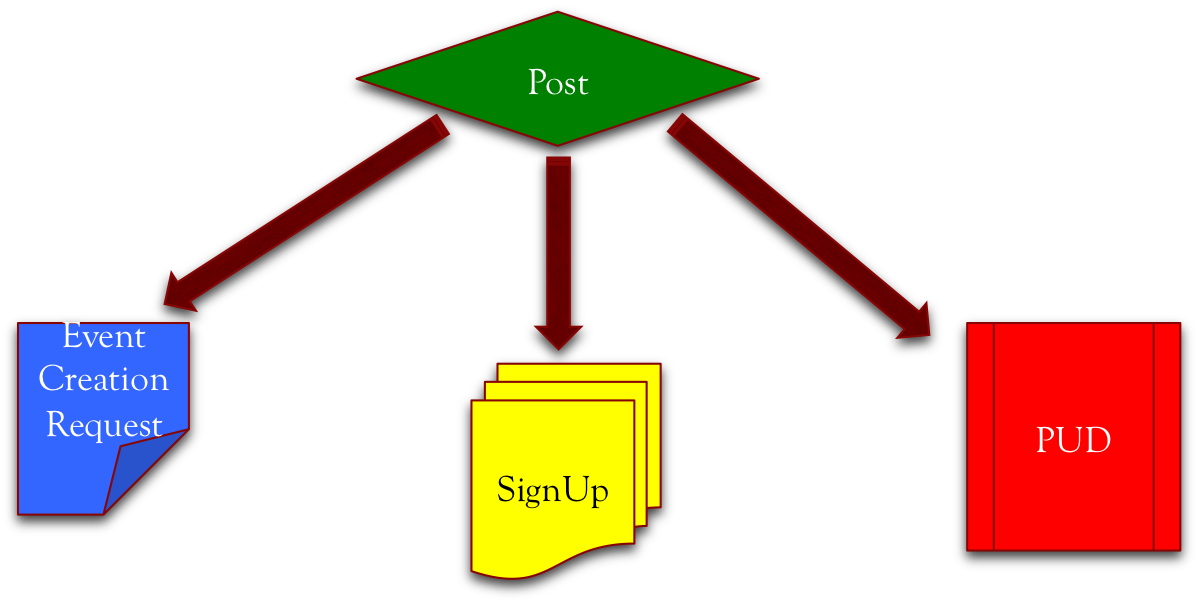
\includegraphics[width=0.4\textwidth]{post_structure.png}
\caption{\label{fig:post_struc}Backend structure for Post with Multi-table Inheritance}
\end{figure}

This design choice comes in extremely handy for sharing. Because a \emph{Signups} object is treated as a \emph{Post} object, we can just use the sharing mechanism already implemented for \emph{Post}. 

A little bit more on the back-end database schema for \emph{Slot Signups}, each \emph{Signups} object consists of a \emph{Signup Sheet} which has one or more \emph{TimeBlock} objects which in turn has a set of \emph{Slot} objects (See Fig. \ref{fig:signup}). This is a very natural choice for the structure based on the project requirement. When creating a \emph{SignUp Sheet} object, the corresponding \emph{TimeBlock} objects are also created and \emph{Slot} objects are created based on the \emph{minimum duration} specified by the owner. Having \emph{Slot} object that is of the \emph{minimum duration} is very useful especially when we try to combine slots. For example, if the user requests for all 30-minute slots when the \emph{minimum duration} is 15 minutes, we can combine 2 consecutive slots to meet the request.


\begin{figure}[h]
\centering
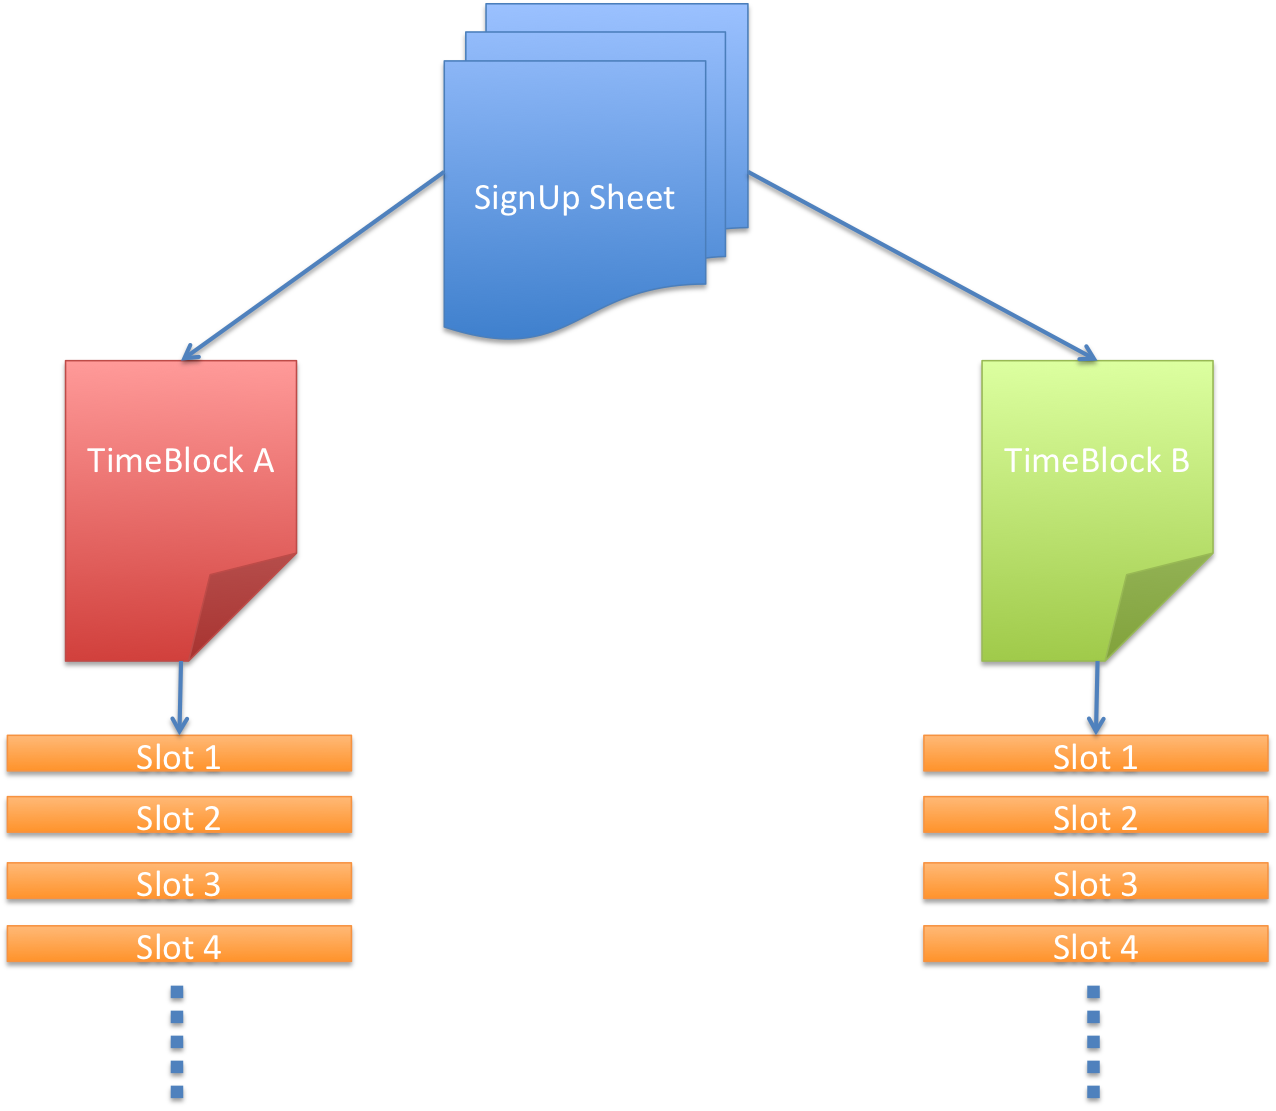
\includegraphics[width=0.4\textwidth]{signup.png}
\caption{\label{fig:signup} Backend structure for \emph{Slot Signups} model}
\end{figure}



\subsection{Freetime Requests}

Freetime requests are at the core of this evolution's features. In this section, we will discuss the implementation and design of freetime, shedding light on the front end and back end modules.

\subsubsection{High-Level Description \& Front-end}

Freetime requests were made using a form, just like the many other functions of Kalendr. The corresponding form allows the user to choose the time slot duration (in hours and minutes), the day range (M-Su), and the time range (0:00 - 23:59). In the case that the freetime request is recurring, by activating the form switch, the user will be able to choose a date range as well. Before submitting the form, the user is able to pick which individuals' schedules they would like to know about.

The freetime summaries are visualized on a screen very similar to the "pudscreen" from evolution II. On this screen, we see individual conflicts and the details of each conflict - user, event, and meta details. The conflicts are not grouped by owners, and instead provide a expansive, deliberately overwhelming view, flooding the user with information. This screen can be accessed by clicking the check button.

As required by the evolution, the user has the capability to create a new event request from the summary page. Because of the way that we implemented groups and sharing, we decided that users cannot request freetimes of groups, since the existence of a certain group does not guarantee that the main user has visible posts from the group. Whereas, in our system, if the user is following another individual, then he or she is guaranteed to have visibility (limited or otherwise) to that specific individual's shared posts.

All of the freetime .html markup is located within account.html and logic concerning freetime requests is handled by \emph{find-freetime.controller.js and conflicts.controller.js}. The structures of these controllers were very similar to the controllers of previous features. Obviously certain changes had to be made to derive the required functionality, but at this stage, it is safe to say that the front-end JavaScript controllers have a common, basic skeleton. The lack of database manipulation and the use of fleeting http POST calls simplified the debugging and testing processes.

\subsubsection{Freetime Back-end Design and Implementation}

First, we will make precise how some of the requirements are interpreted, before explaining the design. As mentioned previously, a user can only specify a set of users whom he or she is ``following", since we have chosen groups to be one-way. Also, when specifying a one-time event, the time range refers to the specified weekdays, starting from tomorrow until a week from the day the request was made. For example, if the user made the request on a Wednesday, and asked for the conflicts on Tuesday, Wednesday, Thursday, then the system will return conflicts on the upcoming Thursday, Tuesday, Wednesday, in that order. And finally, the events that are considered when searching for conflicts are those that either: the specified user has created and has shared with the requesting user; or, some unspecified user has shared with both the specified user and the requesting user, and the specified user has confirmed the event creation request.

In the design of this new feature, like with every other new feature we have added up to this point, adding the free time search was done by creating a new Django app. That is, we write subclasses of {\tt Model}, {\tt ModelSerializer}, and {\tt ModelViewSet} to represent the data definition, serialization, and processing for the API call, respectively. We decided to follow this standard template of a new app in our project, despite something unique to only the free time feature: there are no new database tables, nor any type of additional persistent state required. By doing so, we maintain a regularity, or symmetry, across all of the backend modules for more readability, even though the subclasses extended are not being used as intended by the original designers. We also preserve the same separation of concerns into the three different modules that has worked well for us in the other apps, and has been flexible to changes.

As for weaknesses, the worst is with the datetime manipulation. Given the inconvenient representations chosen in the past, a very large portion of the new code written in the free time modules is with converting and manipulating datetimes of events. This is bad for a few reasons. One, this functionality does not belong in modules for free time. Two, the conversions of event times into a more convenient format should not occur at the time of a free time request. And three, the conversions must be done every time a free time request is made and are redundant, since the conversions are not stored. The purpose of doing it the way we did was to avoid making changes to event representations, since by this point in time, there are many dependencies in the program on events, and the potential of breaking something else was likely and scary. The implication is that we will have to deal with duplicated code in the modules that do require significant datetime processing.


\section{Individual Contributions}
\subsection{Ellango}
Ellango was responsible for implementing the backend for the finding free times feature. In development, he took an approach of writing and testing from the bottom up. That is, he followed an iterative procedure, starting with the lowest-order functions with no dependencies, testing them, and then building up with writing and testing higher-order functions that depend on the already tested code. Thus, at each step, he was able to make the assumption that all previously written code was correct. This allowed interpretation of all errors in the tests to be caused by faulty code isolated in the current function being tested. He found Django's unit testing framework very helpful in setting up fake databases with particular states.

A constraint Ellango dealt with was avoiding side-effects of his development. That is, he did not change the functionality of any other feature in developing free times. In particular, he would have found it useful to change the way datetimes were being used for events, but avoided doing so to avoid any conflicts with the team members working on slot signups during the same time, who had certain assumptions on how datetimes were being used.

Ellango met with his team to make sure there were no misunderstandings between the front-end and back-end regarding data formats. He also interacted with them on Facebook to plan working times and ask and answer short questions. Ellango also used Asana with his team to plan and divide tasks. With our team using Asana, we could ensure accountability for every task that we needed to accomplish.

\subsection{David}
David implemented all the back-end functionality for the new \emph{Signup} feature. He was also responsible for most of the implementation and debugging in the front-end and back-end communication. He worked closely with Benson to implement the \emph{Signup} feature, asking what would be the best way to serve data to the front-end and communicating constraints on the back-end.

He designed the back-end schema for \emph{Signups} and chose the hierarchical structure showed in Fig. \ref{fig:signup}. He learned and utilized the multi-table inheritance to greatly simplify the implementation of the new \emph{Signups} feature. Specifically, the use of multi-table inheritance enabled the team to reuse the entire sharing mechanism that was implemented in evolution 1 and 2. In order to make sure multi-table inheritance would fulfill the needs, he first conducted experiments by building a few simple Django models and seeing what the resulting database schema looked like. 

He generated and analyzed many traces of data flow between the front-end and the back-end. Analysis and interpretation of those data proved to be helpful in debugging and showing that the system is correctly implemented. 

In order to overcome the constraints of the Django REST Framework's serializer (described in Section 3.2.2). He studied the source code of the serializer class and took advantage of the \emph{context-passing} and \emph{SerializerMethodField} features in the serializer class. 

\subsection{Pritam}
Pritam was the mastermind behind the freetime front-end. He used PUD code as scaffolding for freetime functionality. He wrote the controllers to obtain input from the user and package the data into a format that was easily manipulated in the back-end. With directives, Pritam was able to display freetime summaries in a relatively intuitive manner. He also became more comfortable with AngularJS's built in testing framework, and it proved incredibly handy in writing robust code.

He analyzed the traceback for all http GET and POST requests to figure out a way to force pairs of GETs and POSTs to complete in sequence. In the end, it turned out to be impossible, but Pritam figured out another solution. In order to improve the perceived performance of the application, he returned incremental data from POST requests that saved into the database. In this manner he was able to augment data structures in pieces instead of reforming them in their entirety with a GET call. This analysis helped him refactor and simplify a lot of asynchronous callbacks from previous evolutions.

In dealing with realistic constraints, Pritam put UI design decisions on the backburner. This time around, all the requirements, specifically for freetime requests, were completed. It is very obvious that the presentation of the UI is not up to par with previous evolutions. 

Pritam spent time optimizing the styling of Kalendr. Work was put into making the application more responsive to screen size changes, thereby retaining user-friendliness and visual flow. He also made use of bleeding-edge libraries - such as Angular Material - that simplify UI creation and provide a much more consistent feel across the application.

Pritam communicated with his team through Facebook and class, and was diligent in organizing meeting times and booking rooms to work in. 


\subsection{Benson}
Benson focused primarily on the development of front end modules for Slot Signups both on the owner and receivers' end. Much of the front end implementation followed suit from the first two evolutions. He also introduced functionality of new UI elements into forms, providing for a more fluid interface. 

Although much of the front end implementation was predictable, he ran into many date-time issues from hacky solutions he implemented in previous evolutions. More specifically, date and time fields cannot be shown in a readable format to the user if fetched directly from the server. The Datetime Python library also doesn't provide the user with a user-friendly timestamp. Therefore, he decided to write a hacky solution in the back end in Evolution I to provide a legible date, stored as a chracter field rather than a Datetime field, on each calendar post. This definitely convoluted datetime manipulations that were ubiquitous in this evolution.

In retrospect, in spite of popular opinion, he should've considered processing date-time fields in the front end. This would've not only paved a consistent and maintainble pathway for date-time manipulations in the back end, but would've also incurred less overhead. This could've been implemented using popular Javascript libraries such as Moment.js. 

Lastly, he communicated with team members through meetings, Facebook messages and posts, and the use of Asana.


\end{document}
